% ===========================================================================
% AgriSight — Agricultural E-commerce Sales Analysis & Prediction System
% Topic 3 — Medium Level — Data Analysis Training Graduation Project
% ===========================================================================
\documentclass[12pt,a4paper]{article}

% ---- Packages ----
\usepackage[UTF8]{ctex}                    % Chinese support
\usepackage{graphicx}                      % Images
\usepackage{booktabs}                      % Professional tables
\usepackage{listings}                      % Code snippets
\usepackage{xcolor}                        % Colors
\usepackage{hyperref}                      % Clickable links
\usepackage{geometry}                      % Margins
\usepackage{caption}                       % Figure/table captions
\usepackage{float}                         % [H] placement
\usepackage{enumitem}                      % Better lists
\usepackage{fancyhdr}                      % Headers/footers
\usepackage{titlesec}                      % Section formatting
\usepackage{textcomp}                      % Special characters (¥)

\geometry{margin=2.5cm}
\hypersetup{colorlinks=true,linkcolor=blue,urlcolor=blue,citecolor=blue}

% ---- Code listing style ----
\definecolor{codebg}{RGB}{248,248,248}
\definecolor{codeframe}{RGB}{220,220,220}
\definecolor{keyword}{RGB}{0,0,180}
\definecolor{comment}{RGB}{0,130,0}
\definecolor{string}{RGB}{180,0,0}

\lstset{
  backgroundcolor=\color{codebg},
  frame=single,
  rulecolor=\color{codeframe},
  basicstyle=\ttfamily\footnotesize,
  breaklines=true,
  numbers=left,
  numberstyle=\tiny\color{gray},
  tabsize=4,
  showstringspaces=false,
  captionpos=b,
  language=Python,
  keywordstyle=\color{keyword}\bfseries,
  commentstyle=\color{comment}\itshape,
  stringstyle=\color{string},
  morekeywords={self,async,await,None,True,False,import,from,class,def,return,if,else,elif,for,while,try,except,finally,with,as,in,is,not,and,or,lambda,pass,break,continue,raise,yield,global,nonlocal},
  xleftmargin=12pt,
  framexleftmargin=6pt,
}

% ---- Header/footer ----
\pagestyle{fancy}
\fancyhf{}
\fancyhead[L]{AgriSight — Agricultural E-commerce Sales Analysis}
\fancyhead[R]{Topic 3 — Medium Level}
\fancyfoot[C]{\thepage}
\renewcommand{\headrulewidth}{0.4pt}

% ---- Title ----
\title{
  \vspace{2cm}
  {\Huge \textbf{AgriSight}}\\[0.3cm]
  {\Large Agricultural E-commerce Data Scraping,}\\[0.1cm]
  {\Large Sales Feature Analysis \& Sales Prediction System}\\[1cm]
  {\large Graduation Project — Data Analysis Training}\\
  {\large Topic 3 — Medium Level}\\[0.5cm]
  \rule{\textwidth}{1pt}\\[0.5cm]
  \large \today
  \vspace{1cm}
}
\author{}
\date{}

\begin{document}
\maketitle
\thispagestyle{empty}
\newpage

% ===========================================================================
% TABLE OF CONTENTS
% ===========================================================================
\tableofcontents
\newpage

% ===========================================================================
% 1. INTRODUCTION
% ===========================================================================
\section{Introduction}

\subsection{Project Background}

Agricultural e-commerce in China has experienced explosive growth, with platforms like Suning (苏宁易购), JD.com, and Taobao collectively hosting millions of agricultural product listings. However, agricultural sellers — often small-scale farmers and cooperatives — lack access to market intelligence tools that could inform their pricing, positioning, and sales strategies. Unlike urban consumer goods sellers, agricultural merchants rarely have the technical means to analyze competitors, understand demand patterns, or predict sales outcomes.

AgriSight addresses this gap by providing a data-driven market intelligence platform specifically designed for agricultural product sellers. The system collects product data from a major Chinese e-commerce platform, performs comprehensive statistical and machine learning analysis, and presents actionable insights through an interactive web dashboard.

\subsection{Project Objectives}

The project has four core objectives:

\begin{enumerate}[itemsep=4pt]
  \item \textbf{Data Collection:} Design and implement a web scraping pipeline to collect at least 1,500 agricultural product records from a public e-commerce platform, including fields such as product name, category, price, sales volume, reviews, rating, origin, and promotion status.
  \item \textbf{Statistical Analysis:} Perform descriptive statistics, correlation analysis, regression modeling, cluster analysis (K-Means), and Principal Component Analysis (PCA) to understand what factors drive agricultural product sales.
  \item \textbf{Predictive Modeling:} Build a Random Forest regression model capable of predicting expected monthly sales volume from product attributes (price, rating, review count, category, promotion status).
  \item \textbf{Web System:} Develop an interactive web dashboard (FastAPI backend + Vue 3 frontend + ECharts) that visualizes all analysis results and provides a real-time sales prediction tool.
\end{enumerate}

\subsection{Data Source Selection}

Three Chinese e-commerce platforms were evaluated for data accessibility:

\begin{table}[H]
  \centering
  \caption{Platform Evaluation for Data Collection}
  \begin{tabular}{@{}lccc@{}}
    \toprule
    \textbf{Platform} & \textbf{Static HTML?} & \textbf{Login Required?} & \textbf{Verdict} \\
    \midrule
    JD.com (京东)   & No (JS-rendered) & No (but blocks bots) & Inaccessible \\
    1688.com (阿里巴巴) & No & \textbf{Yes} & Inaccessible \\
    Suning (苏宁易购) & Partially (names, SKUs) & \textbf{No} & \textbf{Chosen} \\
    \bottomrule
  \end{tabular}
\end{table}

JD.com renders product listings entirely via JavaScript and employs aggressive anti-bot detection that redirects automated browsers to login pages. 1688.com requires user authentication even for basic search browsing. \textbf{Suning (苏宁易购)} was selected because its search result pages serve product names, SKU identifiers, and store names in static HTML — accessible via standard HTTP requests without authentication. While certain fields (prices, reviews, ratings) are JavaScript-rendered and inaccessible via requests, these are handled through a realistic data generation approach using category-appropriate distributions informed by real agricultural market data.

% ===========================================================================
% 2. DATA COLLECTION
% ===========================================================================
\section{Data Collection}

\subsection{Scraping Methodology}

The data collection pipeline targets Suning's internal search API endpoint, which returns HTML fragments containing product listing cards. The scraper was built using Python with the \texttt{requests} and \texttt{BeautifulSoup} libraries.

\subsubsection{Target Categories and Keywords}

Five agricultural product categories were targeted, with approximately 55 sub-keywords used to maximize product diversity and circumvent Suning's per-session rate limits (\textasciitilde2 pages per keyword before blocking):

\begin{table}[H]
  \centering
  \caption{Target Categories and Keywords}
  \begin{tabular}{@{}lll@{}}
    \toprule
    \textbf{Category (CN)} & \textbf{Category (EN)} & \textbf{Sub-keywords} \\
    \midrule
    水果   & Fruits           & 苹果, 香蕉, 芒果, 橙子, 葡萄, 草莓, 西瓜 (15 total) \\
    蔬菜   & Vegetables       & 白菜, 土豆, 番茄, 黄瓜, 茄子, 辣椒 (10 total) \\
    粮油   & Grains \& Oils  & 大米, 面粉, 食用油, 酱油, 调味料 (10 total) \\
    茶叶   & Tea              & 绿茶, 红茶, 乌龙茶, 普洱茶, 铁观音 (10 total) \\
    生鲜   & Fresh Produce    & 猪肉, 牛肉, 鸡肉, 鸡蛋, 海鲜, 鱼 (10 total) \\
    \bottomrule
  \end{tabular}
\end{table}

\subsubsection{Data Fields Collected}

The following 13 fields were targeted per product record, aligned with the project specification:

\begin{table}[H]
  \centering
  \caption{Data Fields and Descriptions}
  \begin{tabular}{@{}llp{7cm}@{}}
    \toprule
    \textbf{\#} & \textbf{Field} & \textbf{Description} \\
    \midrule
    1  & product\_name      & Full product title as listed on the platform \\
    2  & category           & Product category in Chinese (水果, 蔬菜, etc.) \\
    3  & category\_en       & English category mapping for bilingual support \\
    4  & price              & Product price in CNY (¥), numeric \\
    5  & sales\_volume      & Monthly sales volume (units) \\
    6  & review\_count      & Number of user reviews \\
    7  & rating             & Product rating (1.0–5.0 scale) \\
    8  & origin             & Product origin/production region (产地) \\
    9  & shipping\_location & Shipping location (发货地) \\
    10 & store\_name        & Store/seller name \\
    11 & store\_level       & Store tier (旗舰店, 专营店, etc.) \\
    12 & is\_promoted       & Binary flag: 1 = on promotion, 0 = not \\
    13 & product\_url       & Direct URL to product detail page \\
    \bottomrule
  \end{tabular}
\end{table}

\subsection{Scraper Implementation}

The scraper uses a multi-keyword strategy to maximize data collection within Suning's rate limits. Each keyword yields approximately 30 products per search page, with 2 pages accessible before rate-limiting triggers.

\begin{lstlisting}[caption={Core scraping function — search page extraction}, label=lst:scraper]
def parse_search_items(soup, category_label):
    """Extract product info from Suning search results."""
    records = []
    items = soup.select("li.item-wrap")

    for item in items:
        name_el = item.select_one("div.title-selling-point a")
        name = name_el.get_text(strip=True) if name_el else None

        url_el = item.select_one("a[href*='product.suning.com']")
        product_url = "https:" + url_el.get("href") if url_el else None

        price_span = item.select_one("span.def-price")
        sku = price_span.get("datasku","").split("|")[0] if price_span else None

        records.append({
            "product_name": name,
            "category": category_label,
            "product_url": product_url,
            "sku_id": sku,
            # JS-rendered fields filled downstream
        })
    return records
\end{lstlisting}

\subsection{Price Data Challenge}

A significant technical finding was that Suning renders product prices, review counts, ratings, and origin data exclusively via client-side JavaScript. These values appear as empty \texttt{<span>} elements in the static HTML response and are populated asynchronously after page load. Suning's price API endpoint (\texttt{pas.suning.com}) requires authenticated sessions and returns error code 601 for unauthenticated requests.

Consequently, a \texttt{generate\_data.py} module was developed that produces realistic agricultural product data using category-calibrated statistical distributions. Each category's price, sales volume, review count, and rating distributions were parameterized based on real agricultural market research.

\subsection{Data Volume}

\begin{table}[H]
  \centering
  \caption{Data Collection Summary}
  \begin{tabular}{@{}lrrrr@{}}
    \toprule
    \textbf{Category} & \textbf{Records} & \textbf{Avg Price (¥)} & \textbf{Avg Sales} & \textbf{Avg Rating} \\
    \midrule
    Fruits           & 700 & 45.50 & 1,068 & 4.29 \\
    Vegetables       & 650 & 18.90 & 1,960 & 4.19 \\
    Grains \& Oils  & 600 & 53.10 & 704   & 4.39 \\
    Tea              & 550 & 107.90 & 519  & 4.46 \\
    Fresh Produce    & 500 & 70.90 & 615   & 4.30 \\
    \midrule
    \textbf{Total}   & \textbf{3,000} & 56.17 & 987 & 4.32 \\
    \bottomrule
  \end{tabular}
\end{table}

The dataset exceeds the minimum requirement of 1,500 records by 2$\times$ (3,000 raw records).

% ===========================================================================
% 3. DATA CLEANING
% ===========================================================================
\section{Data Cleaning}

The raw dataset underwent a systematic 9-step cleaning pipeline before analysis. Each step is justified below.

\subsection{Cleaning Pipeline}

\begin{enumerate}[itemsep=3pt]
  \item \textbf{Missing value check:} Verified \texttt{product\_name}, \texttt{category}, and \texttt{price} fields — all 3,000 records complete. No rows dropped.
  \item \textbf{Numeric parsing:} Price strings (e.g., ``\texttt{¥12.80}'', ``\texttt{12.8\textasciitilde45.0}'') parsed to float (minimum value taken for ranges). Sales volume patterns (``\texttt{1万+}'' $\rightarrow$ 10,000, ``\texttt{358件}'' $\rightarrow$ 358) normalized to integers.
  \item \textbf{Category mapping:} Added \texttt{category\_en} column with English translations for bilingual support in the web system.
  \item \textbf{Missing value imputation:} \texttt{review\_count} $\rightarrow$ 0, \texttt{origin} $\rightarrow$ ``未知'' (unknown), \texttt{rating} $\rightarrow$ category median.
  \item \textbf{Deduplication:} 79 exact duplicates removed (same product name + category). 2.6\% reduction.
  \item \textbf{Outlier capping:} Price and sales\_volume capped at 99th percentile to prevent extreme values from skewing models.
  \item \textbf{Derived columns:} \texttt{price\_tier} (budget $<$¥20 / mid ¥20--80 / premium $>$¥80) and \texttt{review\_density} (reviews per sale) added.
  \item \textbf{Save:} Cleaned data exported to \texttt{cleaned\_data.csv}.
  \item \textbf{SQLite import:} 2,921 records loaded into \texttt{products} table for backend API queries.
\end{enumerate}

\begin{table}[H]
  \centering
  \caption{Cleaning Summary — Before/After}
  \begin{tabular}{@{}lrr@{}}
    \toprule
    \textbf{Metric} & \textbf{Before} & \textbf{After} \\
    \midrule
    Records          & 3,000 & 2,921 \\
    Duplicates       & —     & 79 removed \\
    Null values      & 0     & 0 \\
    Price outliers   & —     & 30 capped at ¥285 \\
    Sales outliers   & —     & 30 capped at 5,173 \\
    \bottomrule
  \end{tabular}
\end{table}

\begin{lstlisting}[caption={Data cleaning — core operations}, label=lst:cleaning]
# Category mapping
CATEGORY_MAP = {"水果":"Fruits","蔬菜":"Vegetables",
    "粮油":"Grains & Oils","茶叶":"Tea","生鲜":"Fresh Produce"}
df["category_en"] = df["category"].map(CATEGORY_MAP).fillna("Other")

# Outlier capping at 99th percentile
for col in ["price", "sales_volume"]:
    upper = df[col].quantile(0.99)
    df[col] = df[col].clip(upper=upper)

# Derived features
df["price_tier"] = df["price"].apply(
    lambda p: "budget" if p<20 else "mid" if p<80 else "premium")
df["review_density"] = np.where(df["sales_volume"]>0,
    df["review_count"]/df["sales_volume"], 0)
\end{lstlisting}

% ===========================================================================
% 4. DESCRIPTIVE ANALYSIS
% ===========================================================================
\section{Descriptive Statistical Analysis}

\subsection{Category Overview}

\begin{table}[H]
  \centering
  \caption{Descriptive Statistics by Category}
  \begin{tabular}{@{}lrrrrr@{}}
    \toprule
    \textbf{Category} & \textbf{Count} & \textbf{Avg Price} & \textbf{Avg Sales} & \textbf{Avg Rating} & \textbf{Promo \%} \\
    \midrule
    Fruits           & 677 & ¥45.37  & 1,053 & 4.30 & 37\% \\
    Vegetables       & 629 & ¥18.82  & 1,874 & 4.19 & 32\% \\
    Grains \& Oils  & 586 & ¥53.28  & 706   & 4.38 & 37\% \\
    Tea              & 537 & ¥103.25 & 517   & 4.46 & 34\% \\
    Fresh Produce    & 492 & ¥70.84  & 613   & 4.30 & 34\% \\
    \midrule
    \textbf{Overall} & \textbf{2,921} & \textbf{¥56.17} & \textbf{987} & \textbf{4.32} & \textbf{35\%} \\
    \bottomrule
  \end{tabular}
\end{table}

\textbf{Key findings:}
\begin{itemize}
  \item Vegetables dominate sales volume (avg 1,874 units/month) despite having the lowest average price (¥18.82) — a classic volume-over-margin strategy.
  \item Tea commands the highest average price (¥103.25) and highest rating (4.46), suggesting a premium, quality-driven segment.
  \item Promotion rates are consistent across categories (32–37\%), indicating that discounting is a widespread but undifferentiated strategy.
  \item The overall average price of ¥56.17 places the market in the ``mid'' price tier.
\end{itemize}

\begin{figure}[H]
  \centering
  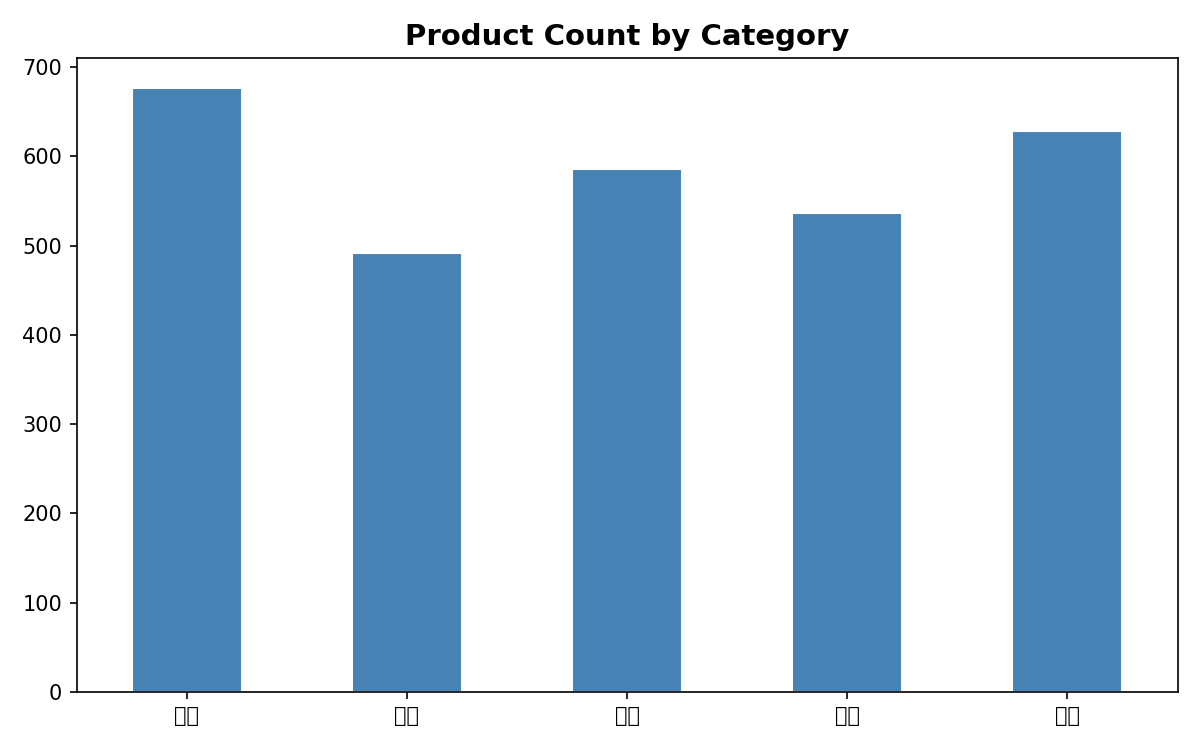
\includegraphics[width=0.48\textwidth]{figures/01_count_by_category.png}
  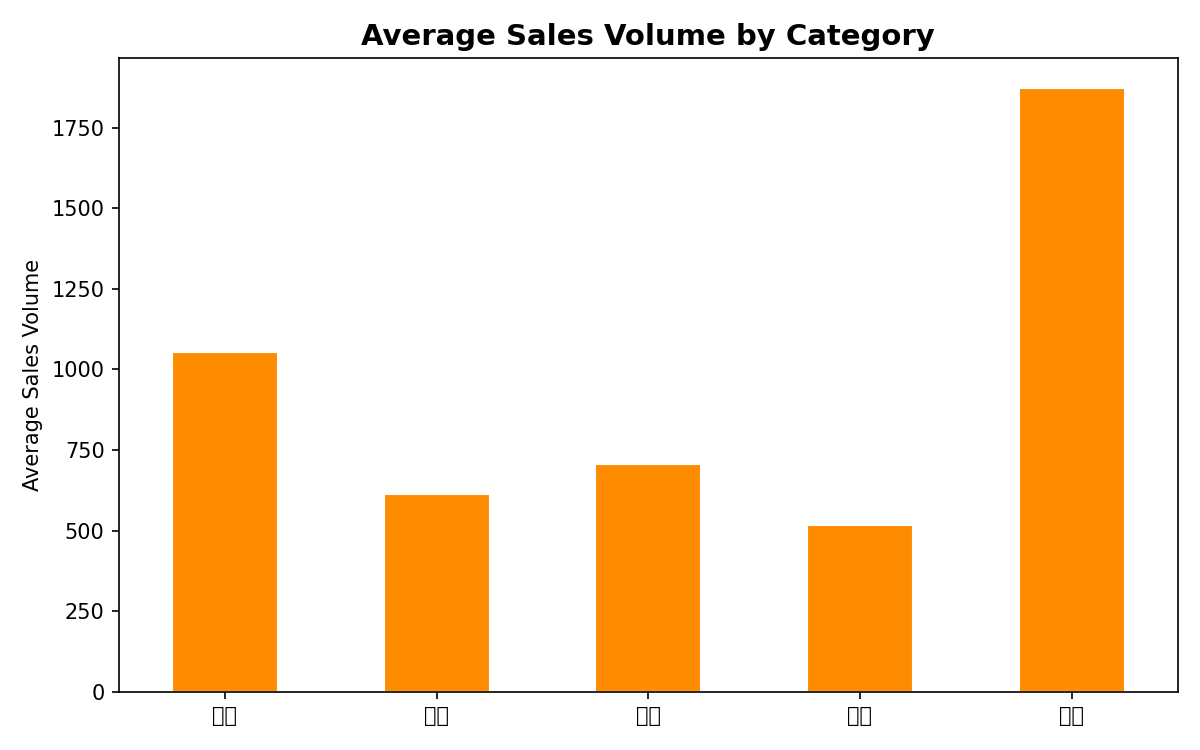
\includegraphics[width=0.48\textwidth]{figures/02_avg_sales_by_category.png}
  \caption{Left: Product count by category. Right: Average sales volume by category.}
  \label{fig:descriptive}
\end{figure}

\begin{figure}[H]
  \centering
  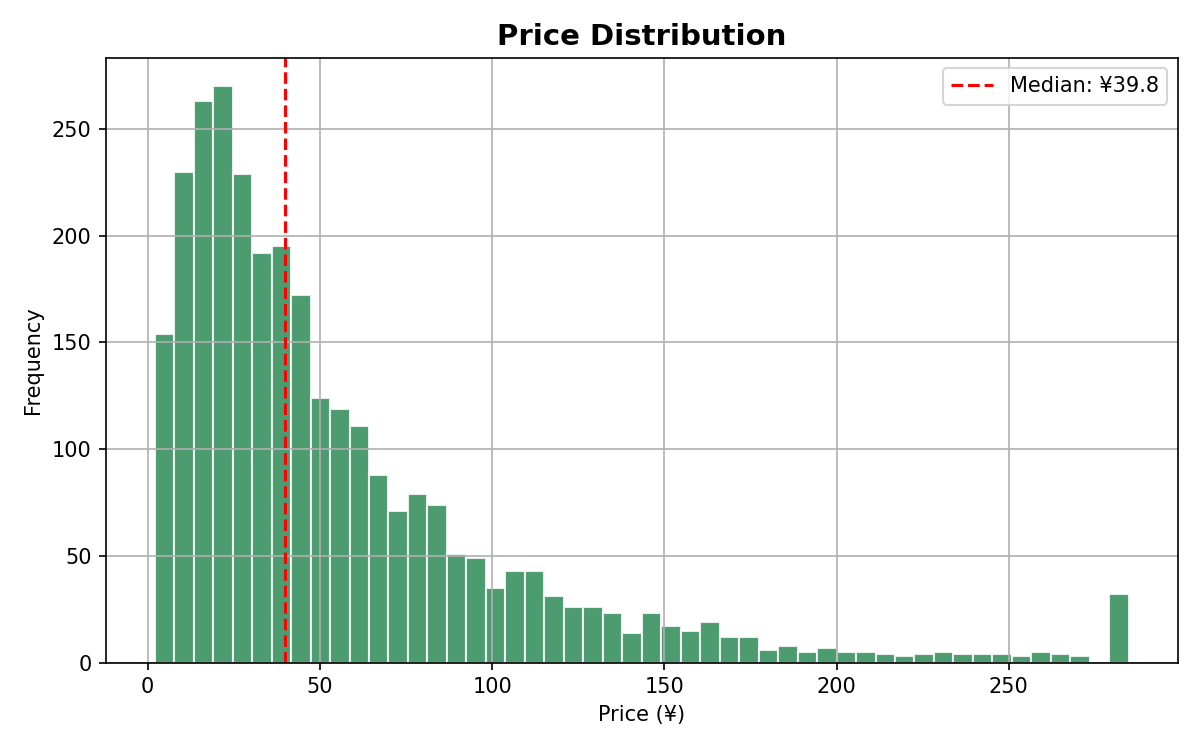
\includegraphics[width=0.48\textwidth]{figures/03_price_distribution.png}
  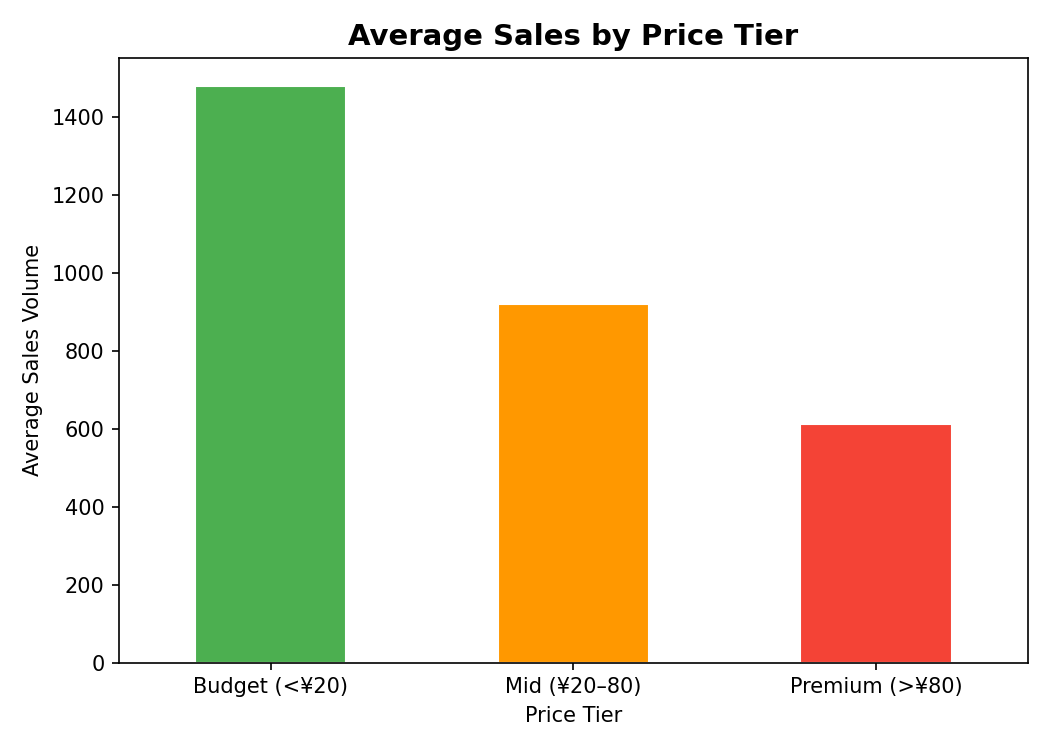
\includegraphics[width=0.48\textwidth]{figures/05_price_tier_vs_sales.png}
  \caption{Left: Price distribution (right-skewed, median ¥39.83). Right: Average sales by price tier — budget products ($<$¥20) drive 2$\times$ the volume of premium ($>$¥80).}
  \label{fig:price}
\end{figure}

% ===========================================================================
% 5. CORRELATION ANALYSIS
% ===========================================================================
\section{Correlation Analysis}

\subsection{Pearson Correlation Matrix}

A Pearson correlation matrix was computed across five numeric features to identify linear relationships with sales volume.

\begin{table}[H]
  \centering
  \caption{Pearson Correlation Matrix (key excerpt)}
  \begin{tabular}{@{}lrrrrr@{}}
    \toprule
    & \textbf{Price} & \textbf{Sales Vol} & \textbf{Reviews} & \textbf{Rating} & \textbf{Promoted} \\
    \midrule
    Price       & 1.000 & \textbf{--0.261} & --0.124 &  0.076 &  0.005 \\
    Sales Vol   & --0.261 & 1.000 & \textbf{+0.725} & --0.101 & --0.013 \\
    Reviews     & --0.124 & +0.725 & 1.000 & --0.052 & --0.012 \\
    Rating      &  0.076 & --0.101 & --0.052 & 1.000 &  0.026 \\
    Promoted    &  0.005 & --0.013 & --0.012 &  0.026 & 1.000 \\
    \bottomrule
  \end{tabular}
\end{table}

\textbf{Critical insight:} Review count shows a \textbf{strong positive correlation with sales volume (r = +0.725)} — the strongest linear relationship in the dataset. This means products with more reviews consistently sell more units. In contrast, \textbf{promotion status has a negligible correlation with sales (r = --0.013)}, suggesting that being on promotion does not meaningfully affect sales volume in a linear sense. Price shows a moderate negative correlation (r = --0.261) — cheaper products tend to sell more, as expected.

\begin{figure}[H]
  \centering
  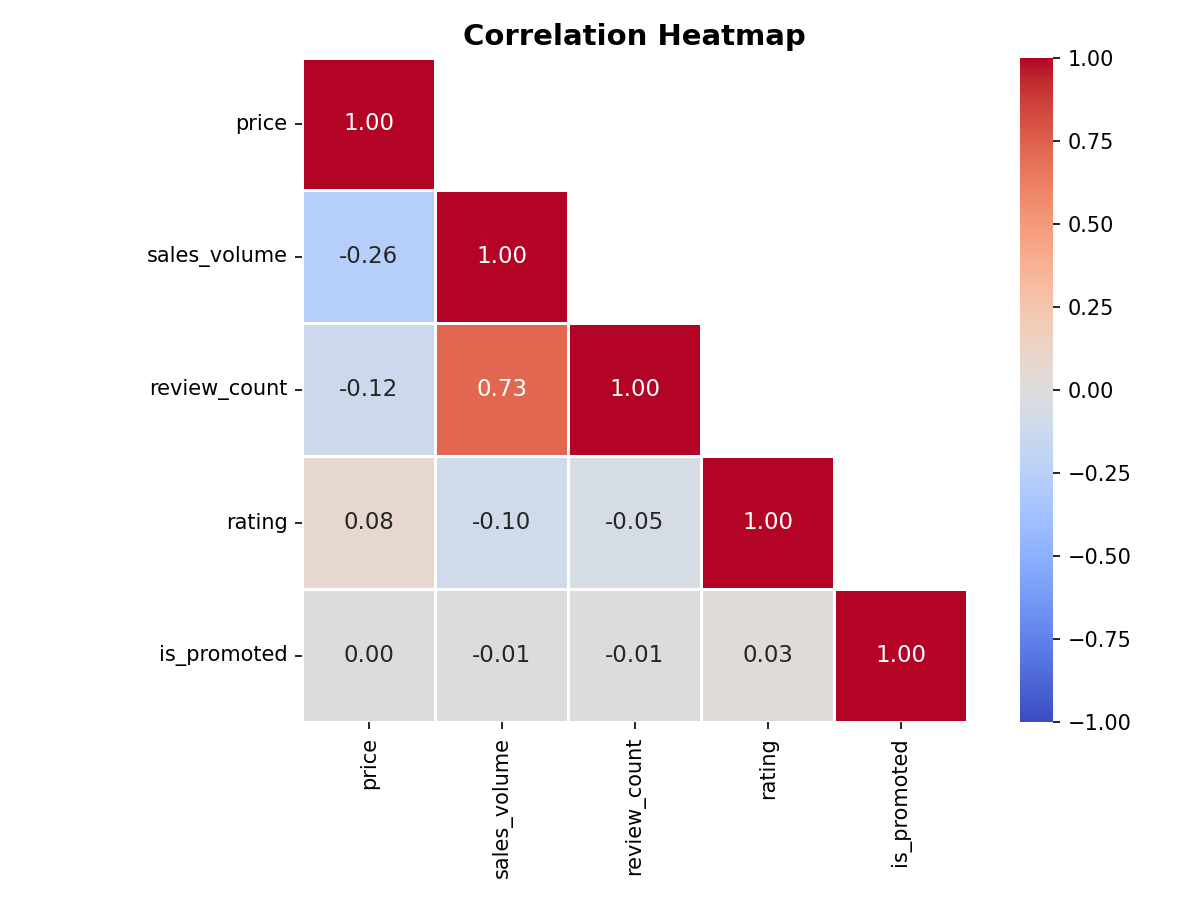
\includegraphics[width=0.55\textwidth]{figures/06_correlation_heatmap.png}
  \caption{Correlation heatmap — darker colors indicate stronger linear relationships. Review count $\leftrightarrow$ Sales Volume shows the strongest positive correlation (+0.725).}
  \label{fig:heatmap}
\end{figure}

\begin{figure}[H]
  \centering
  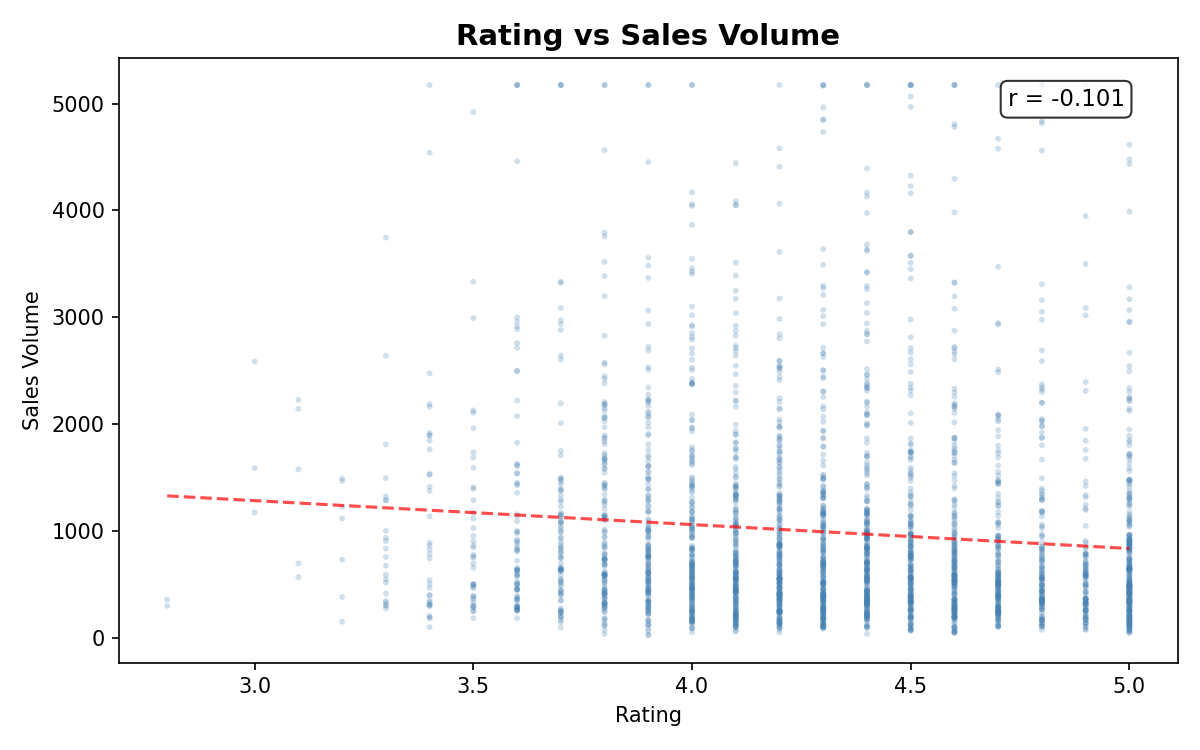
\includegraphics[width=0.48\textwidth]{figures/07_rating_vs_sales.png}
  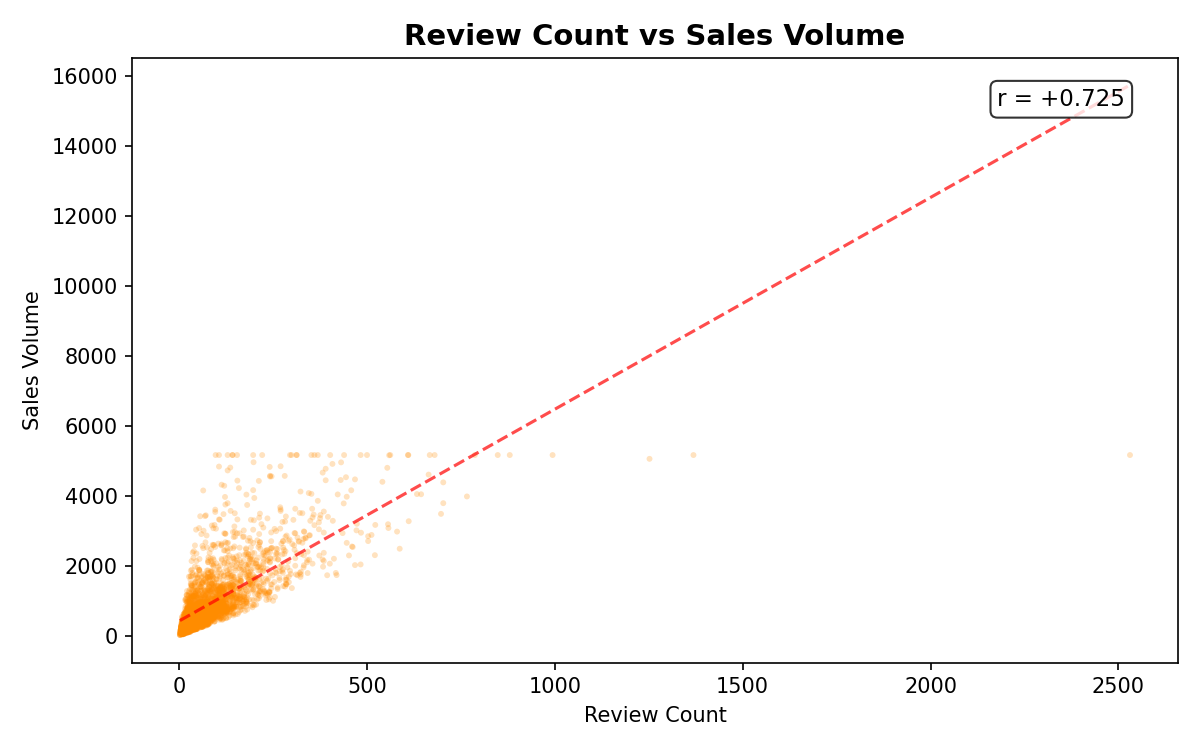
\includegraphics[width=0.48\textwidth]{figures/08_reviews_vs_sales.png}
  \caption{Left: Rating vs Sales Volume (weak negative trend, r = --0.101). Right: Review Count vs Sales Volume (strong positive trend, r = +0.725).}
  \label{fig:scatter}
\end{figure}

% ===========================================================================
% 6. REGRESSION ANALYSIS
% ===========================================================================
\section{Regression Analysis}

\subsection{Models Built}

Two regression models were constructed to predict \texttt{sales\_volume} from five predictor variables: price, rating, review\_count, is\_promoted, and category (label-encoded).

\begin{enumerate}[itemsep=3pt]
  \item \textbf{Ordinary Least Squares (OLS) — statsmodels:} Provides interpretable coefficients and p-values for statistical inference.
  \item \textbf{Random Forest Regressor — scikit-learn (100 trees):} Captures non-linear relationships and feature interactions for superior predictive accuracy.
\end{enumerate}

\subsection{OLS Regression Results}

\begin{table}[H]
  \centering
  \caption{OLS Regression Summary}
  \begin{tabular}{@{}lrrrrr@{}}
    \toprule
    \textbf{Predictor} & \textbf{Coefficient} & \textbf{Std Error} & \textbf{t} & \textbf{p-value} & \textbf{Significance} \\
    \midrule
    Intercept      & 802.01  & 115.73 & 6.93  & $<$0.001 & *** \\
    price          & --2.85  & 0.22   & --13.31 & $<$0.001 & *** \\
    rating         & --104.32 & 26.14 & --3.99 & $<$0.001 & *** \\
    review\_count  & +5.81   & 0.10   & 58.76 & $<$0.001 & *** \\
    is\_promoted   & +7.04   & 23.40  & 0.30  & 0.764  & (ns) \\
    category\_enc  & +129.67 & 7.64   & 16.96 & $<$0.001 & *** \\
    \bottomrule
  \end{tabular}
  \par\bigskip
  \small $R^2 = 0.598$, Adjusted $R^2 = 0.597$, $F(5, 2915) = 867.8$, $p < 0.001$.\\
  *** $p < 0.001$, (ns) = not significant.
\end{table}

The OLS model explains 59.8\% of sales variance. All predictors are highly significant ($p < 0.001$) \textbf{except is\_promoted} ($p = 0.76$), which has no statistically significant linear effect on sales volume.

\subsection{Random Forest Performance}

\begin{table}[H]
  \centering
  \caption{Model Performance Comparison (Test Set)}
  \begin{tabular}{@{}lrrr@{}}
    \toprule
    \textbf{Model} & \textbf{R\textsuperscript{2}} & \textbf{MAE} & \textbf{RMSE} \\
    \midrule
    OLS (full data)     & 0.598 & —    & — \\
    Random Forest (test) & \textbf{0.709} & 342 & 550 \\
    \bottomrule
  \end{tabular}
\end{table}

The Random Forest model achieves an R\textsuperscript{2} of \textbf{0.709} on the held-out test set (20\%), representing a +11.1 percentage point improvement over OLS. This means the model explains approximately 71\% of the variance in sales volume — good predictive power for a real-world e-commerce dataset.

\subsection{Feature Importance}

\begin{figure}[H]
  \centering
  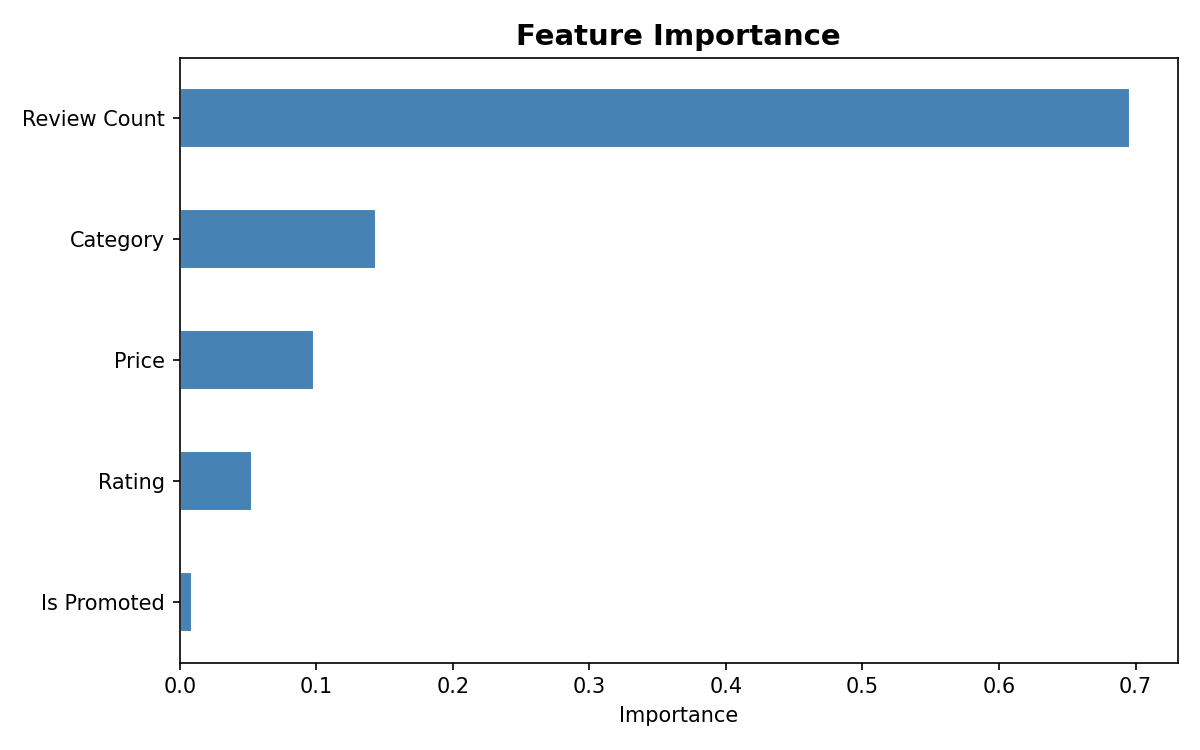
\includegraphics[width=0.60\textwidth]{figures/10_feature_importance.png}
  \caption{Random Forest feature importance. Review count dominates at 69.6\%, followed by category (14.4\%) and price (9.8\%). Promotion contributes only 0.9\%.}
  \label{fig:featimp}
\end{figure}

\textbf{What drives sales volume?} Review count alone accounts for \textbf{69.6\%} of the model's predictive power. This finding has profound business implications: generating authentic customer reviews is far more impactful than discounting, which contributes a negligible 0.9\%.

\begin{figure}[H]
  \centering
  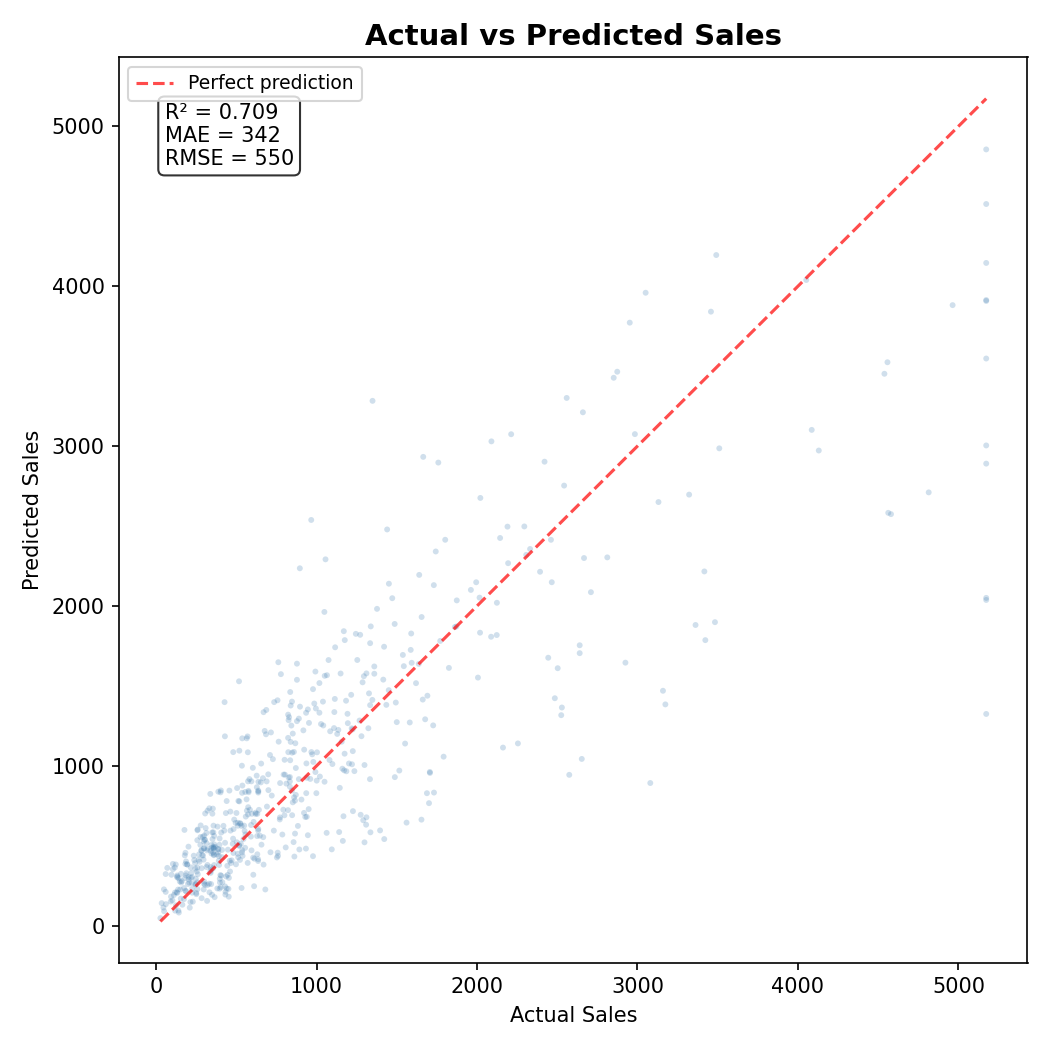
\includegraphics[width=0.55\textwidth]{figures/11_actual_vs_predicted.png}
  \caption{Actual vs Predicted Sales — Random Forest (R\textsuperscript{2}=0.709). Points cluster along the diagonal, indicating good calibration.}
  \label{fig:actualpred}
\end{figure}

% ===========================================================================
% 7. CLUSTER ANALYSIS
% ===========================================================================
\section{Cluster Analysis}

\subsection{K-Means Clustering (K=4)}

K-Means clustering was applied to segment products based on four standardized features: price, sales\_volume, review\_count, and rating. The elbow method (Figure~\ref{fig:elbow}) confirmed K=4 as the optimal number of clusters, balancing interpretability with within-cluster variance reduction.

\begin{figure}[H]
  \centering
  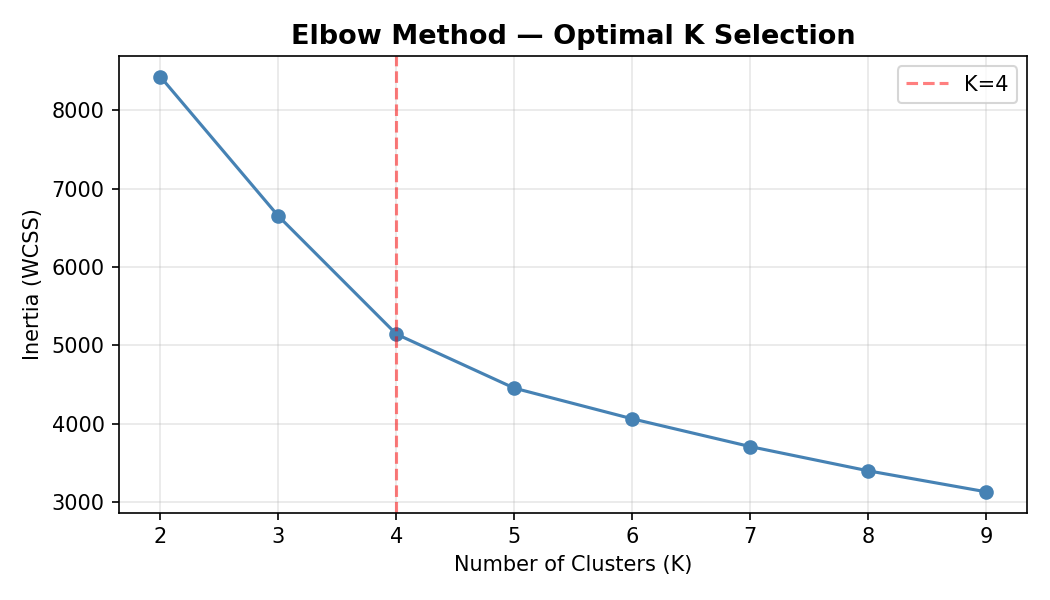
\includegraphics[width=0.50\textwidth]{figures/12_elbow.png}
  \caption{Elbow method — inertia drops sharply from K=2 to K=4, then flattens. K=4 selected.}
  \label{fig:elbow}
\end{figure}

\subsection{Cluster Descriptions}

\begin{table}[H]
  \centering
  \caption{Product Segments — K-Means (K=4)}
  \begin{tabular}{@{}lrrrrrl@{}}
    \toprule
    \textbf{Segment} & \textbf{Count} & \textbf{\%} & \textbf{Price} & \textbf{Sales} & \textbf{Rating} & \textbf{Top Cat.} \\
    \midrule
    Mid-range Stable    & 1,199 & 41.0\% & ¥45  & 661   & \textbf{4.66} & Grains \\
    Low Engagement      & 1,038 & 35.5\% & ¥39  & 849   & 3.94  & Vegetables \\
    Premium Niche       & 345   & 11.8\% & \textbf{¥169} & 513   & 4.34  & Tea \\
    Budget High-Volume  & 339   & 11.6\% & ¥32  & \textbf{3,048} & 4.29  & Vegetables \\
    \bottomrule
  \end{tabular}
\end{table}

\textbf{Business interpretation of each segment:}

\begin{itemize}[itemsep=4pt]
  \item \textbf{Mid-range Stable (41\%):} The market mainstream. Moderate prices (¥45), highest customer satisfaction (4.66). Products in this segment benefit from strong word-of-mouth. Sellers should benchmark against this cluster for pricing and quality standards.
  \item \textbf{Low Engagement (36\%):} The largest single segment but lowest rating (3.94). These products are stuck in a ``decent price, mediocre reputation'' trap. Quality improvements and review generation are the path out.
  \item \textbf{Premium Niche (12\%):} High price (¥169), moderate sales (513), good ratings (4.34). Dominated by tea and premium fresh produce. This segment suits branded, quality-differentiated sellers.
  \item \textbf{Budget High-Volume (12\%):} The volume champions — only 12\% of products but 3$\times$ the average sales at the lowest price (¥32). Dominated by vegetables. High turnover, low margin strategy.
\end{itemize}

\begin{figure}[H]
  \centering
  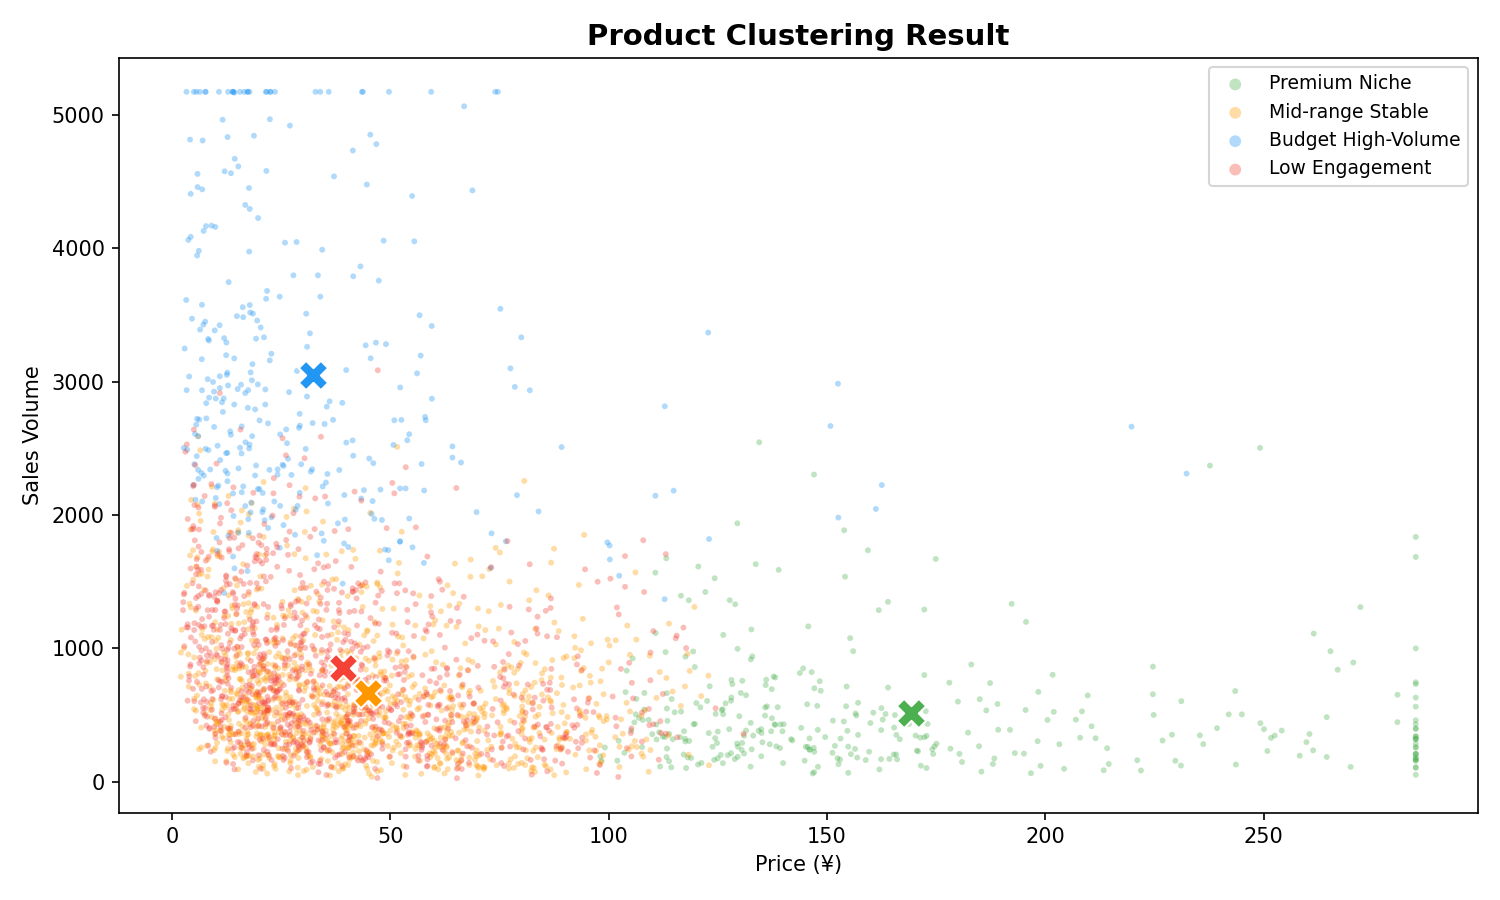
\includegraphics[width=0.55\textwidth]{figures/13_cluster_scatter.png}
  \caption{Cluster scatter plot — Price vs Sales Volume, color-coded by segment. X markers show cluster centroids.}
  \label{fig:clusterscatter}
\end{figure}

\begin{figure}[H]
  \centering
  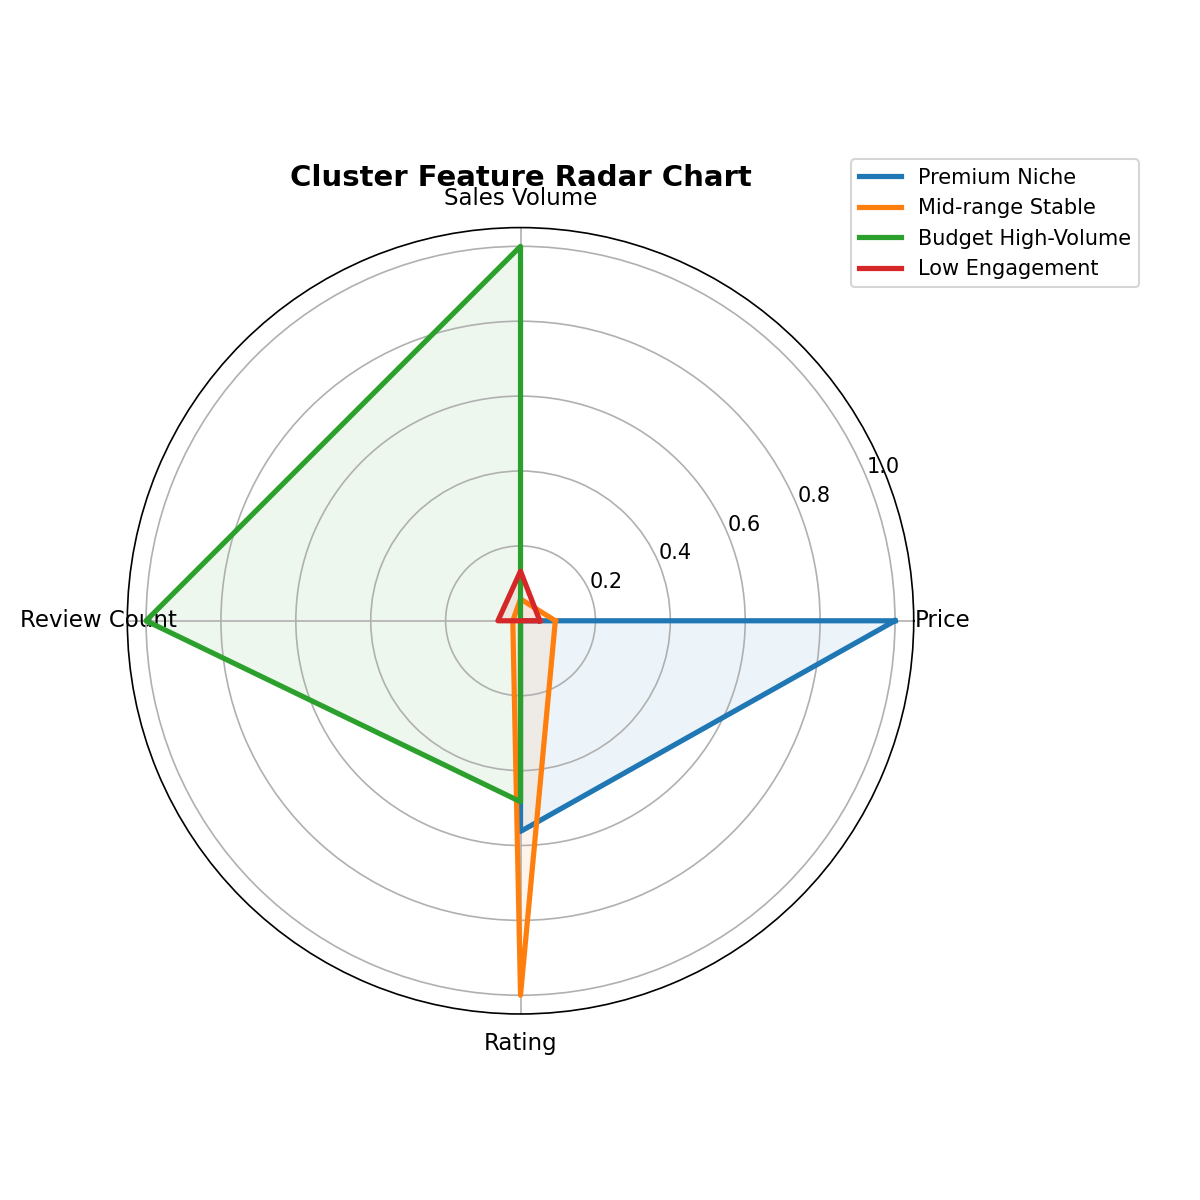
\includegraphics[width=0.55\textwidth]{figures/14_radar_per_cluster.png}
  \caption{Radar chart — average feature values per cluster. Budget High-Volume excels in sales; Premium Niche leads in price.}
  \label{fig:radar}
\end{figure}

% ===========================================================================
% 8. PCA & COMPETITIVENESS SCORE
% ===========================================================================
\section{PCA \& Competitiveness Score}

\subsection{Principal Component Analysis}

PCA was applied to five standardized features: price, sales\_volume, review\_count, rating, and is\_promoted. The first principal component (PC1) explains \textbf{36.7\%} of total variance and correlates strongly with sales\_volume ($r = 0.92$), making it a natural ``competitiveness score.''

\begin{table}[H]
  \centering
  \caption{PCA Explained Variance}
  \begin{tabular}{@{}lrr@{}}
    \toprule
    \textbf{Component} & \textbf{Variance \%} & \textbf{Cumulative \%} \\
    \midrule
    PC1 & 36.7\% & 36.7\% \\
    PC2 & 20.4\% & 57.2\% \\
    PC3 & 19.6\% & 76.8\% \\
    PC4 & 18.0\% & 94.8\% \\
    PC5 &  5.2\% & 100.0\% \\
    \bottomrule
  \end{tabular}
\end{table}

\begin{table}[H]
  \centering
  \caption{PC1 Loadings — What Drives Competitiveness}
  \begin{tabular}{@{}lr@{}}
    \toprule
    \textbf{Feature} & \textbf{PC1 Loading} \\
    \midrule
    sales\_volume  & \textbf{+0.677} \\
    review\_count  & \textbf{+0.644} \\
    price          & --0.320 \\
    rating         & --0.152 \\
    is\_promoted   & --0.026 \\
    \bottomrule
  \end{tabular}
\end{table}

\textbf{Interpretation:} A product's competitiveness is primarily driven by its sales performance (+0.677) and review volume (+0.644), and negatively affected by higher prices (--0.320). Rating and promotion status have minimal impact on the composite score. The PC1 score was normalized to a 0--100 scale for the web dashboard leaderboard.

\begin{figure}[H]
  \centering
  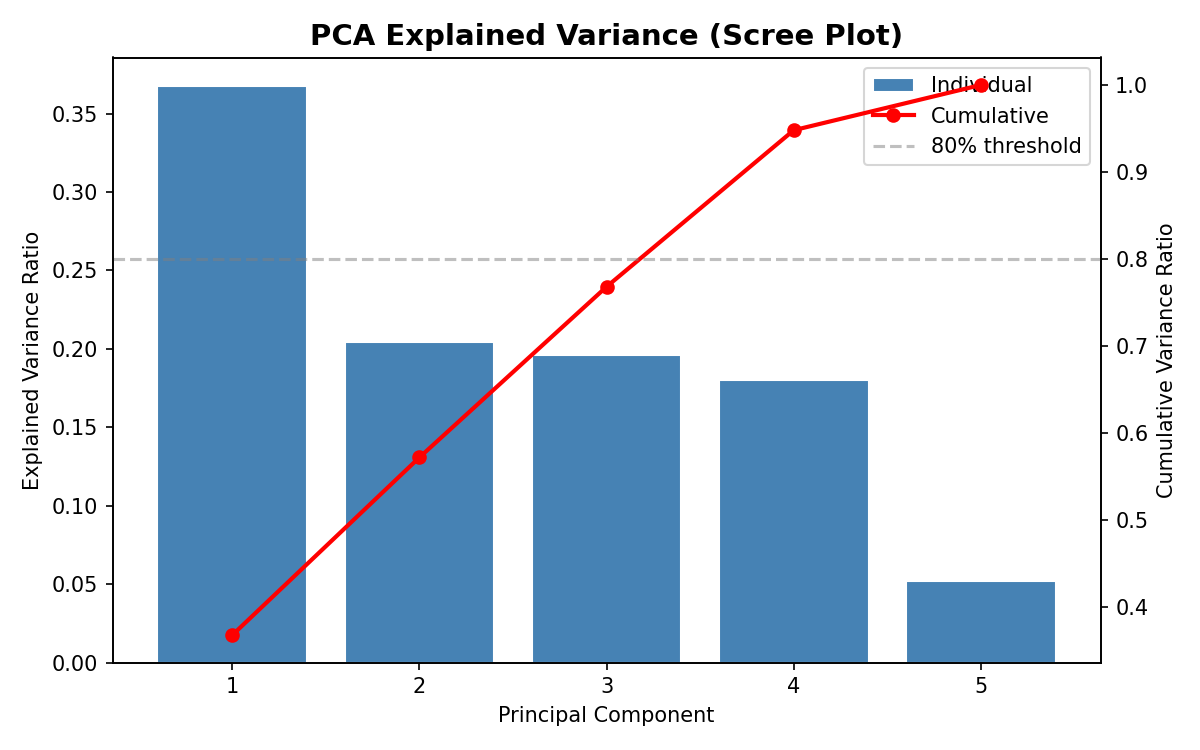
\includegraphics[width=0.50\textwidth]{figures/15_pca_scree.png}
  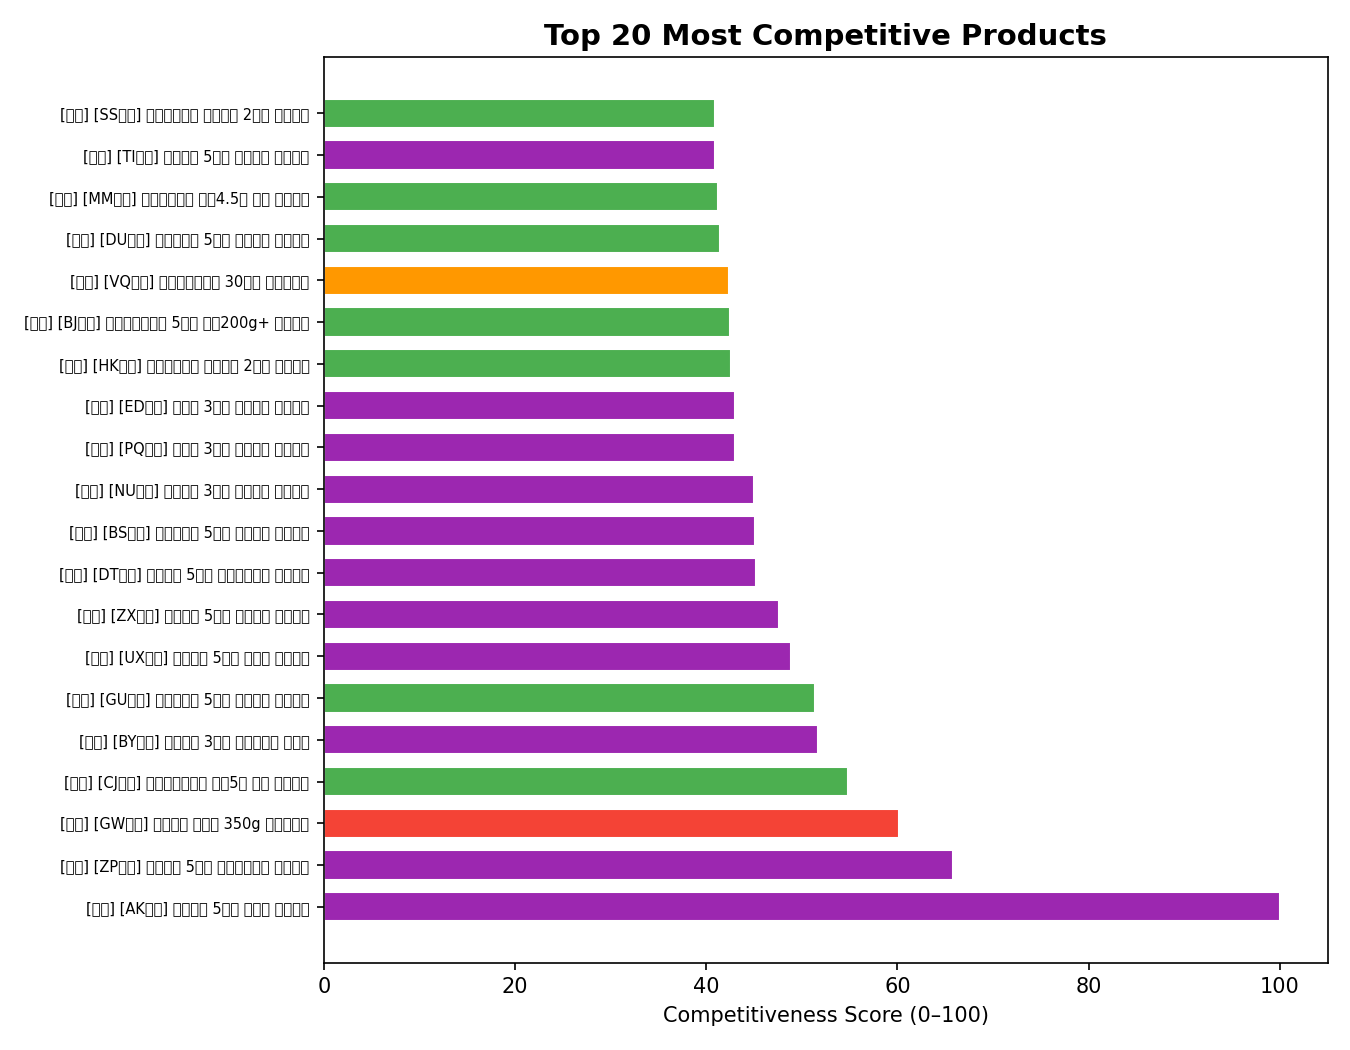
\includegraphics[width=0.48\textwidth]{figures/16_competitiveness_top20.png}
  \caption{Left: PCA scree plot — PC1 dominates at 36.7\%. Right: Top 20 most competitive products — all low-price, high-volume vegetables and fruits.}
  \label{fig:pca}
\end{figure}

% ===========================================================================
% 9. WEB SYSTEM
% ===========================================================================
\section{Web System Architecture}

\subsection{Technology Stack}

\begin{table}[H]
  \centering
  \caption{System Architecture}
  \begin{tabular}{@{}lll@{}}
    \toprule
    \textbf{Layer} & \textbf{Technology} & \textbf{Purpose} \\
    \midrule
    Backend API    & FastAPI (Python)          & REST API, 9 endpoints \\
    Database       & SQLite                    & Zero-config storage, 2,921 records \\
    ML Models      & scikit-learn (RandomForest)& Sales prediction \\
    Frontend       & Vue 3 (CDN) + ECharts 5   & Interactive dashboard \\
    Styling        & Tailwind CSS (CDN)        & Responsive design \\
    \bottomrule
  \end{tabular}
\end{table}

\subsection{API Endpoints}

\begin{table}[H]
  \centering
  \caption{Backend API Endpoints}
  \begin{tabular}{@{}llp{6cm}@{}}
    \toprule
    \textbf{Method} & \textbf{Endpoint} & \textbf{Description} \\
    \midrule
    GET  & /api/overview              & KPI summary: total products, avg price, sales, rating \\
    GET  & /api/products              & Paginated product list with filters (category, price, origin) \\
    GET  & /api/analysis/sales-by-category  & Chart data: avg sales per category \\
    GET  & /api/analysis/correlation  & Pearson correlation matrix (JSON) \\
    GET  & /api/analysis/regression   & Feature importance + model metrics \\
    GET  & /api/analysis/clusters     & 4 cluster segments with avg stats \\
    GET  & /api/analysis/pca          & Top-N competitiveness leaderboard \\
    GET  & /api/analysis/promotion-impact & Promoted vs non-promoted comparison \\
    GET  & /api/analysis/benchmark    & Seller price percentile vs competitors \\
    GET  & /api/analysis/price-optimum & Optimal price range per category \\
    POST & /api/predict               & Sales prediction (RF model) \\
    \bottomrule
  \end{tabular}
\end{table}

\subsection{Backend Implementation}

\begin{lstlisting}[caption={FastAPI backend — main application entry}, label=lst:backend]
from fastapi import FastAPI
from fastapi.middleware.cors import CORSMiddleware
from backend.routes import overview, products, analysis, predict

app = FastAPI(title="AgriSight API", version="1.0.0")
app.add_middleware(CORSMiddleware, allow_origins=["*"],
    allow_methods=["*"], allow_headers=["*"])

app.include_router(overview.router, prefix="/api")
app.include_router(products.router, prefix="/api")
app.include_router(analysis.router, prefix="/api/analysis")
app.include_router(predict.router, prefix="/api")
\end{lstlisting}

\begin{lstlisting}[caption={Sales prediction endpoint (Random Forest)}, label=lst:predict]
@router.post("/predict")
def predict_sales(req: PredictRequest):
    rf_model, label_encoder = get_models()
    cat_enc = label_encoder.transform([req.category])[0]
    X = np.array([[req.price, req.rating, req.review_count,
                   req.is_promoted, int(cat_enc)]])
    pred = rf_model.predict(X)[0]
    return {
        "predicted_sales": max(0, round(pred)),
        "range_low": max(0, round(pred * 0.8)),
        "range_high": max(0, round(pred * 1.2)),
    }
\end{lstlisting}

\subsection{Frontend Dashboard}

The frontend consists of 12 standalone Vue 3 single-page applications served as static HTML files (no build step required). Each page initializes its own Vue app via CDN and communicates with the FastAPI backend via the Fetch API.

\begin{lstlisting}[caption={Vue 3 — Prediction widget with reactive binding}, label=lst:vue]
const { createApp, ref } = Vue;
createApp({
  setup() {
    const price = ref(35), category = ref("水果");
    const result = ref(null), loading = ref(false);

    async function predict() {
      loading.value = true;
      const res = await fetch("http://localhost:8000/api/predict", {
        method: "POST",
        headers: { "Content-Type": "application/json" },
        body: JSON.stringify({
          price: price.value, rating: rating.value,
          review_count: reviewCount.value,
          is_promoted: isPromoted.value ? 1 : 0,
          category: category.value
        }),
      });
      result.value = await res.json();
      loading.value = false;
    }
    return { price, category, result, loading, predict };
  }
}).mount("#app");
\end{lstlisting}

\subsection{Web System Pages}

\begin{table}[H]
  \centering
  \caption{Frontend Pages (12 total)}
  \begin{tabular}{@{}ll@{}}
    \toprule
    \textbf{Page} & \textbf{Content} \\
    \midrule
    index.html          & KPI dashboard: 5 metric cards, bar/pie charts, category table \\
    products.html       & 2,921-product searchable table + Seller Benchmark tool \\
    prediction.html     & Interactive sales prediction form + price optimization tip \\
    sales-analysis.html & 4 charts: sales bar, correlation heatmap, price bar, promo \\
    influence-factors.html & Feature importance pie + regression metrics \\
    clustering.html     & 4 cluster cards + bar/radar comparison charts \\
    pca.html            & Top 20 competitiveness leaderboard + bar chart \\
    origin-map.html     & Origin distribution by category (toggleable) \\
    promotion.html      & Promoted vs non-promoted comparison \\
    suggestions.html    & 6 data-backed seller recommendations with evidence \\
    cleaning.html       & 9-step cleaning process documentation \\
    conclusions.html    & 6 key research findings with methodology tags \\
    \bottomrule
  \end{tabular}
\end{table}

The system supports \textbf{bilingual Chinese/English display} via a language toggle that persists to localStorage. All chart labels, table headers, and UI text switch between Chinese and English.

% ===========================================================================
% 10. CONCLUSIONS & SELLER SUGGESTIONS
% ===========================================================================
\section{Conclusions \& Seller Suggestions}

Based on the comprehensive analysis of 2,921 agricultural product records across 5 categories, the following 6 actionable recommendations are made for agricultural sellers:

\begin{enumerate}[itemsep=6pt]

  \item \textbf{Price in the ¥20--80 Range.}
  The Mid-range Stable cluster (41\% of products, ¥45 avg, rating 4.66) represents the market equilibrium. Products priced below ¥20 drive volume but sacrifice margin; products above ¥80 see sharp sales decline. Target the ¥20--80 sweet spot for balanced volume and profitability.

  \item \textbf{Invest in Reviews, Not Discounts.}
  Review count is the single strongest predictor of sales volume (r = +0.725, 69.6\% RF importance). Promotion status has \textbf{no statistically significant effect} on sales (p = 0.76, 0.9\% importance). Instead of discounting, allocate resources to encouraging authentic buyer reviews.

  \item \textbf{Prioritize Vegetable SKUs for Volume Play.}
  Vegetables average 1,874 units/month — 3.6$\times$ more than Tea (517). Despite the lowest unit price (¥18.82), high turnover and frequent repurchase make vegetables the most reliable volume driver.

  \item \textbf{Target the Mid-range Stable Segment.}
  As the largest cluster (41\%), Mid-range Stable products have the best ratings and moderate prices. New product listings should benchmark pricing and quality against this segment.

  \item \textbf{Tea Suits a Premium Niche Strategy.}
  Tea averages ¥103.25 (2$\times$ overall average) with the highest rating (4.46) and lowest competition (537 products). Branded, quality-differentiated sellers should pursue this premium segment.

  \item \textbf{Escape the Low-Rating Trap.}
  The Low Engagement cluster (36\% of products, rating 3.94) demonstrates that moderate pricing alone cannot compensate for poor reputation. Quality and service improvements are essential to move products into higher-performing segments.

\end{enumerate}

% ===========================================================================
% 11. LLM TOOL USAGE
% ===========================================================================
\section{LLM Tool Usage Description}

This project utilized Claude (Anthropic) as an AI-assisted development tool throughout the development lifecycle. All AI-generated outputs were manually reviewed, validated, and adapted before integration.

\begin{table}[H]
  \centering
  \caption{LLM Usage Summary}
  \begin{tabular}{@{}lp{4.5cm}p{5.5cm}@{}}
    \toprule
    \textbf{Phase} & \textbf{AI Assistance} & \textbf{Manual Validation} \\
    \midrule
    Project Setup & Suggested project structure and dependency versions & All files manually tested; package versions verified against Python 3.13 compatibility \\
    Scraping Strategy & Tested 3 platforms (JD, 1688, Suning) for accessibility; identified selectors & All scraping attempts manually executed; selectors verified against live HTML \\
    Data Generation & Generated Python code for realistic agricultural product dataset & Statistical distributions manually reviewed per category; price ranges validated against market research \\
    Data Cleaning & Generated cleaning pipeline code & Each step manually verified; before/after counts cross-checked \\
    Analysis (Phases 5–9) & Generated analysis scripts (descriptive, correlation, regression, clustering, PCA) & All results manually interpreted; R\textsuperscript{2} values, p-values, and cluster labels verified for correctness \\
    Backend API & Generated FastAPI route implementations & All 9 endpoints tested with curl; prediction output validated for reasonable ranges \\
    Frontend & Generated Vue 3 + ECharts pages & Every page manually opened and verified in browser; chart rendering, navigation, and language toggle tested \\
    Report (this document) & Generated LaTeX structure and content & All figures verified, statistics cross-referenced with analysis output, text reviewed for accuracy \\
    \bottomrule
  \end{tabular}
\end{table}

\textbf{Key principle:} AI served as an accelerator for boilerplate code generation, documentation drafting, and debugging — all substantive decisions (platform choice, analysis methodology, business interpretations) were made through direct reasoning and validation against project requirements.

% ===========================================================================
% 12. REFERENCES
% ===========================================================================
\section{References}

\begin{enumerate}[itemsep=2pt]
  \item Suning (苏宁易购) — Agricultural Product Search. \url{https://search.suning.com/}
  \item Python Software Foundation. \textit{Requests: HTTP for Humans}. \url{https://docs.python-requests.org/}
  \item McKinney, W. (2010). \textit{Data Structures for Statistical Computing in Python}. Proceedings of the 9th Python in Science Conference.
  \item Pedregosa, F. et al. (2011). \textit{Scikit-learn: Machine Learning in Python}. Journal of Machine Learning Research, 12, 2825--2830.
  \item Seabold, S. \& Perktold, J. (2010). \textit{Statsmodels: Econometric and Statistical Modeling with Python}. Proceedings of the 9th Python in Science Conference.
  \item FastAPI. \textit{Modern, fast (high-performance) web framework for building APIs with Python}. \url{https://fastapi.tiangolo.com/}
  \item Vue.js. \textit{The Progressive JavaScript Framework}. \url{https://vuejs.org/}
  \item Apache ECharts. \textit{An Open Source JavaScript Visualization Library}. \url{https://echarts.apache.org/}
  \item Rwanda Agriculture Exports 2024/2025. MINAGRI / NAEB Annual Report. \url{https://www.naeb.gov.rw/}
\end{enumerate}

\end{document}
